\section{Security and the Internet Protocol}
Es gibt viele verschiedene Technologien, um die Kommunikation �ber das Internet sicherer zu machen. Viele davon sind aber an eine bestimmte Anwendung gekoppelt (in diesem Fall werden die Sicherheitsmechanismen auf dem Application Layer bereitgestellt).
\paragraph{Beispiele}
\begin{itemize}
	\item PGP ("`Pretty Good Privacy"') f�r die Verschl�sselung von E-Mails und Browser-basierte Authentifizierung
	\item SSL ("`Secure Sockets Layer"') f�r die Verschl�sselung des Datenverkehrt zwischen Web-Browser und Web-Server.
\end{itemize}
Nat�rlich ist das f�r grosse Firmen oder f�r einen ISP (Internet Service Provider) nicht geeignet, da morgen andere Applikationen �ber die heutigen Netzwerke laufen k�nnten.
\subsection{Possible Threats in the Internet}
VPNs m�ssen mindestens die folgenden drei Anforderungen erf�llen:
\begin{itemize}
	\item Authentication (Die Person, mit der man kommuniziert, ist die, f�r die sie sich ausgibt)
	\item Confidentiality \& Privacy (Niemand soll den Datenverkehrt belauschen k�nnen)
	\item Integrity (Daten d�rfen w�hrend der �bertragung nicht ver�ndert werden k�nnen)
\end{itemize}
\subsubsection{Spoofing}
Beim Spoofing gibt sich ein Angreifer als jemand anderes aus, indem er Pakete mit einer entsprechenden IP-Source-Adresse statt der eigenen versieht. Es ist eine allgemeine Tatsache, dass eine IP-Source-Adresse nicht vertrauensw�rdig ist.

\begin{figure}[!htb]
	\centering
	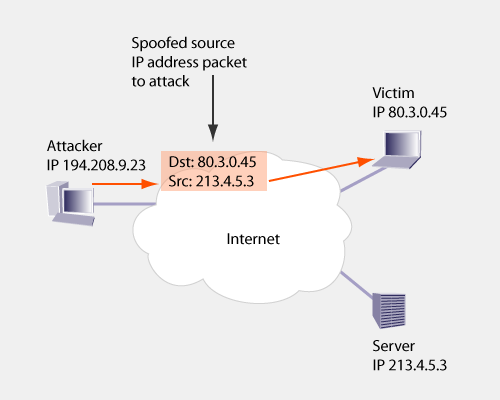
\includegraphics[width=0.50\textwidth]{figure_2_3.png}
\end{figure}
\subsubsection{Session Hijacking / Man in the Middle Attack}
Ein Hacker kann sich "`in die Mitte eines Kommunikationsweges setzen,"' und die Kommunikationspartner jeweils glauben lassen, er sei das Gegen�ber. Er kann s�mtliche Datenpakete filtern und manipulieren. Es reicht daher nicht aus, einen Kommunikations-partner \textit{einmal} zu identifizieren, sondern es sollte jede Datenquelle authentifiziert werden.
\begin{figure}[!htb]
	\centering
	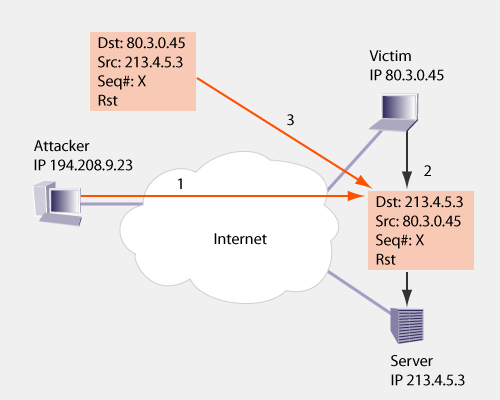
\includegraphics[width=0.50\textwidth]{figure_2_4.png}
\end{figure}
\subsubsection{Electronic Eavesdropping}
Ein grosser Teil der meisten Netzwerke basiert auf Ethernet LANs. Das Abh�ren solcher Ethernet-Leitungen ist einfach - noch ernster ist die Lage bei Wireless-LANs.
In Ethernet-Netzwerken kann jeder angeschlossene Knoten jedes Paket lesen. Es ist eine Konvention, dass jeder Knoten nur die an ihn adressierten Pakete verarbeitet. Nat�rlich kann ein Ger�t einfach konfiguriert werden, dass es alle Pakete "`sammmelt,"' �ber die Leitung verschickt werden. Physikalisch ist es nicht m�glich, an einem anderen Standort im Netzwerk festzustellen, dass ein Ger�t alle Pakete verarbeitet.